%% LyX 2.0.3 created this file.  For more info, see http://www.lyx.org/.
%% Do not edit unless you really know what you are doing.
\documentclass[english]{article}
\usepackage[T1]{fontenc}
\usepackage[latin9]{inputenc}
\usepackage{geometry}
\geometry{verbose,tmargin=0.75in,bmargin=0.75in,lmargin=0.75in,rmargin=1in}
\usepackage{graphicx}

\makeatletter

%%%%%%%%%%%%%%%%%%%%%%%%%%%%%% LyX specific LaTeX commands.
%% Because html converters don't know tabularnewline
\providecommand{\tabularnewline}{\\}

\makeatother

\usepackage{babel}
\begin{document}
\thispagestyle{empty}

\begin{tabular*}{1\textwidth}{@{\extracolsep{\fill}}lr}
\textbf{ID:} 03 & \textbf{Collaborator \#1:} Last Name, First Name\tabularnewline
\textbf{Name:} Al-Naji, Nader & \textbf{Collaborator \#2:} Last Name, First Name\tabularnewline
\hline 
\end{tabular*}

\medskip{}


\begin{center}
\begin{Large}\textbf{Solution to HW 9, Problem 1}\end{Large}
\par\end{center}

\begin{center}
\begin{large}\textbf{COS 340 - Spring 2012}\end{large}
\par\end{center}

\bigskip{}


% Begin sol%
I pledge my Honor that I have not voilated the Honor code on this exam. Nader Al-Naji
\newline
\newline
Decide whether each of the following statements is true or false. If it is true, give a proof. If it is false, give a counterexample. 
\newline
\newline
\textbf{True or False? If in a simple undirected graph, if $u$ and $v$ are the only vertices of odd degree, then $u$ and $v$ are connected.}
\newline
\newline
True. We prove this by showing that any simple undirected graph must have an even number of vertices with odd degree. Let the set of all vertices be denoted by $X$ in the following computations and the set of all edges be denoted by $E$. We have the fact that:
\newline
\newline
$\sum\limits_{x \in X}^{} deg(x) = 2|E|$. 
\newline
\newline
This is true since each edge contributes one to the degree of two vertices. $2|E|$ is an even number, since it is divisible by 2, by the definition of what it is for a number to be even. Therefore, the sum of the vertex degrees, which is equal to $2|E|$, must also be even. We now break up the sum over vertex degrees on the left-hand side into a sum over vertices with odd degree and a sum over vertices of even degree. Let $Odd$ denote the set of vertices in $X$ with odd degree and let $Even$ denote the set of vertices in $X$ with even degree:
\newline
\newline
$\sum\limits_{x \in X}^{} deg(x) = 2|E| \rightarrow \sum\limits_{o \in Odd}^{} deg(o) + \sum\limits_{e \in Even}^{} deg(e) = 2|E| \rightarrow \sum\limits_{o \in Odd}^{} deg(o) = 2|E| - \sum\limits_{e \in Even}^{} deg(e)$.
\newline
\newline
Now we have some work to do. Our goal is to show that the number on the right is always even and, after doing this, to show that the number on the left can only be even when the number of vertices with odd degree is even. 
\newline
\newline
\textbf{Lemma 1:} the sum of $n$ even numbers is $even$ for all values of $n \geq 0$.
\newline
\newline
An even number $N$ has a factor of two in it by the definition of what it is for a number to be even and so, pulling out this factor, any even number can be written as $2k$ for some $k$. To show that the sum of two even numbers is again even, we take the sum of two even numbers $2k$ and $2m$ where $k$ and $m$ are integers and get:
\newline
\newline
$(2k)+(2m) = 2(k + m)$.
\newline
\newline
Thus, the sum of two even numbers always has a factor of two in it and, therefore, is always even. Applying this result recursively, the sum of $n$ even numbers is always even since the parity never changes.
\newline
\newline
\textbf{Lemma 2: $even - even = even$}
\newline
\newline
This again goes by taking two even numbers $2k$ and $2m$ and performing the operation on them:
\newline
\newline
$2k - 2m = 2 (k - m)$.
\newline
\newline
The result has a factor of two in it and, therefore, is also even.
\newline
\newline
\textbf{Lemma 3: $odd + even = odd$}
\newline
\newline
If we subtract one from an odd number, we get an even number, which we can take a factor of two out of, and so it should be clear that any number that is odd can be written as $2k + 1$ for some $k$. Thus we have that the sum of an odd number $(2k + 1)$ and an even number $2m$ is:
\newline
\newline
$(2k + 1) + (2m) = (2k + 2m) + 1 = 2(k + m) + 1 = 2C + 1$.
\newline
\newline
This final result is an even number plus one and, therefore, is odd.
\newline
\newline
\textbf{Lemma 4: $odd + odd = even$}
\newline
\newline
The proof of this is again straightforward taking two odd numbers $(2k + 1)$ and $(2m + 1)$ and adding:
\newline
\newline
$(2k + 1) + (2m + 1) = (2k + 2m + 2) = 2(k + m + 1)$.
\newline
\newline
Thus, we have that the sum of two odd numbers has a factor of two in it and, therefore, is even.
\newline
\newline
\textbf{Lemma 5:} The sum of an even number of odd numbers is even AND the sum of an odd number of odd numbers is odd.
\newline
\newline
Using the previous lemmas, we know that summing two odd numbers results in an even number and summing an even number with an odd number results in an odd number. Thus, if $n$ is the number of odd numbers to be summed together, the parity of the result changes $n-1$ times, starting with a change from odd to even. Thus if $n$ is $odd$, then the parity will change an even number of times, because $n-1$ is even, and the final result of the sum will be again $odd$. If $n$ is even, then the parity will change an $odd$ number of times, because $n-1$ is odd, and the result will be even.
\newline
\newline
Putting this all together, we have:
\newline
\newline
$\sum\limits_{o \in Odd}^{} deg(o) = 2|E| - \sum\limits_{e \in Even}^{} deg(e) \rightarrow \sum\limits_{o \in Odd}^{} deg(o) = even - even = even$ by Lemmas $1$ and $2$.
\newline
\newline
Thus, using Lemma $5$, if $|Odd|$ is odd, then we will have that $odd = even$, a contradiction. If $|Odd|$ is even, on the other hand, we have that $even = even$ and the equation is consistent. Thus, $|Odd|$ must be even $\rightarrow$ any simple graph must have an even number of $odd$ vertices. 
\newline
\newline
Using this fact, if $u$ and $v$ are not connected, then we will have $2$ subgraphs of $G$ that contain an odd number of vertices with odd degree, a contradiction. Thus if $G$ contains $u$ and $v$ such that these are the only vertices with $odd$ degree, $u$ and $v$ must be connected in order to have all subgraphs contain an even number of vertices with odd degree and avoid this contradiction.
\newline
\newline
\textbf{True or False? If in a simple undirected graph, $u$ and $v$ are the only vertices of even degree, then $u$ and $v$ are connected.}
\newline
\newline
False. Consider an empty graph (no edges between vertices) consisting only of $u$ and $v$. The degree of both vertices is, then, $0$, which is even, and yet there is no path from $u$ to $v$ since the graph is empty. Thus, it is not necessarily true that if $u$ and $v$ are the only vertices of even degree that $u$ and $v$ are connected.
\newline
\newline
\textbf{True or False? There exists a simple undirected connected planar 6-regular graph.}
\newline
\newline
False. First, we show that $|F| \leq 2/3 |E|$ if a graph is planar, where $F, E,$ and $V$ denote the sets of faces, edges, and vertices respectively. Then we show that we have a contradiction with $6-regular$ graphs:
\newline
\newline
In a planar graph, each face has degree at least $3 \rightarrow deg(f_i) \geq 3 \mbox{ } \forall \mbox{ } f_i \in F$. Also note that the sum of the face degrees is $2|E|$ since each edge contributes two face boundaries; these facts were also mentioned in class. Thus, we have:
\newline
\newline
$2|E| = \sum\limits_{f \in F}^{} deg(f) \geq 3|F| \rightarrow |E| \geq 3/2|F| \rightarrow |F| \leq 2/3|E|$.
\newline
\newline
Now we show that we have a contradiction with $6-regular$ graphs. Recall that the sum of vertex degrees is equal to $2|E|$ and note that, since each vertex has degree $6$, the sum of vertex degrees is equal to $6|V|$:
\newline
\newline
$\sum\limits_{v \in V}^{} deg(v) = 6|V| = 2|E| \rightarrow |V| = 1/3|E|$. Now, using Euler's formula, we have:
\newline
\newline
$|V| + |F| = 2 + |E| \rightarrow 1/3|E| + |F| = 2 + |E| \rightarrow |F| = 2 + 2/3|E| \rightarrow |F| > 2/3|E|$, a contradiction.
\newline
\newline
Thus, since $6-regular$ graphs do not obey $|F| \leq 2/3|E|$, a property of all planar graphs, we have a contradiction and, therefore, there cannot exist a simple, undirected, connected, planar $6-regular$ graph.
\newline
\newline
\textbf{True or False? In any graph, the size of a maximum matching is equal to the size of a minimum vertex cover.}
\newline
\newline
False. Consider the following graph:
\newline
\newline
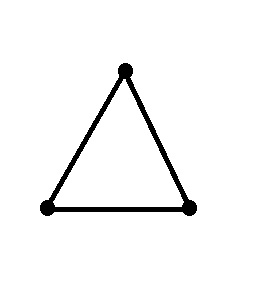
\includegraphics[scale=0.5]{1_4.jpg}
\newline
\newline
A matching is a set of edges that do not overlap at any vertex. For this graph, a matching can consist of at most one edge since including a second edge would cause the edges in the set to overlap at a vertex. Thus, the size of the maximum matching for this graph is $1$. A vertex cover is a set of vertices that ``cover'' all of the edges. For this graph, a single vertex is not enough to cover all the edges: no matter which vertex we choose, we can cover only two edges. Thus, in order to cover all of the edges we need at least two vertices so the size of the minimum vertex cover is $2$. Thus, the size of the maximum matching is not equal to the size of the minimum vertex cover for this graph and so the statement is false in general. The statement is true for bipartite graphs by Konig's Theorem.
% End sol%

\pagebreak{}

\thispagestyle{empty}

\begin{tabular*}{1\textwidth}{@{\extracolsep{\fill}}lr}
\textbf{ID:} 03 & \textbf{Collaborator \#1:} Last Name, First Name\tabularnewline
\textbf{Name:} Al-Naji, Nader & \textbf{Collaborator \#2:} Last Name, First Name\tabularnewline
\hline 
\end{tabular*}

\medskip{}


\begin{center}
\begin{Large}\textbf{Solution to HW 9, Problem 2}\end{Large}
\par\end{center}

\begin{center}
\begin{large}\textbf{COS 340 - Spring 2012}\end{large}
\par\end{center}

\bigskip{}


% Begin sol%
I pledge my Honor that I have not voilated the Honor code on this exam. Nader Al-Naji
\newline
\newline
Prove that every triangle-free (simple undirected) planar graph is $4$-colorable. Do not use the four color theorem.
\newline
\newline
\textbf{Lemma 1: } In any triangle-free simple undirected planar graph, there must exist a vertex with degree $\leq 3$.
\newline
\newline
Because this graph is triangle-free, every face has at least four face boundaries. Further, because every edge contributes two boundaries, we have the following:
\newline
\newline
$2|E| = \sum\limits_{f \in F}^{} deg(f) \geq 4|F| \rightarrow 2|E| \geq 4|F| \rightarrow |E| \geq 2|F|$.
\newline
\newline
Further, since the graph is planar, we can plug into Euler's formula and get:
\newline
\newline
$|V| + |F| = 2 + |E| \rightarrow |F| = 2 + |E| - |V| 
\newline \rightarrow |E| \geq 2|F| \rightarrow |E| \geq 2(2+|E|-|V|) \rightarrow |E| \leq 2|V| - 4$. 
\newline
\newline
And combining this with the fact that the sum of the vertex degree is equal to twice the number of edges, we have:
\newline
\newline
$\sum\limits_{v \in V}^{} deg(v) = 2|E| \rightarrow \frac{\sum\limits_{v \in V}^{} deg(v)}{|V|} = \mbox{average vertex degree} = \frac{2|E|}{|V|}
\newline\rightarrow \mbox{average vertex degree} = \frac{2|E|}{|V|} \leq \frac{4|V| - 8}{|V|} = 4 - 8/|V|
\newline\rightarrow \mbox{average vertex degree} \leq 4 - 8/|V| \rightarrow \mbox{average vertex degree} < 4$.
\newline
\newline
The fact that the average vertex degree, derived above, is strictly less than four allows us to conclude that in any triangle-free simple undirected planar graph, there must exist a vertex with degree $\leq 3$ since otherwise there would be nothing to pull the average down.
\newline
\newline
Using this lemma, we can now construct a simple inductive proof.
\newline
\newline
Let $Q(n) = \mbox{``Any triangle-free simple undirected planar graph with n nodes is 4-colorable''}$.
\newline
\newline
\textbf{Base: } $n = 0, 1, 2, 3, 4$ just to be thorough.
\newline
\newline
Clearly if the graph contains $\leq 4$ vertices, four colors is sufficient to color it since we can just give every vertex its own unique color to ensure no conflicts arise.
\newline
\newline
\textbf{Step: } Assume $Q(n)$ true. Prove $Q(n+1)$.
\newline
\newline
Take any triangle-free simple undirected graph with $n+1$ vertices. By lemma $1$, we know that in this graph there exists a vertex with degree $\leq 3$. So we can find this vertex, pull it and all of its adjacent edges off, color the new graph of size $n$ with four colors by the inductive hypothesis, and then reattach this vertex and color it with a color different than its (at most three) adjacent vertices without introducing any new colors. Thus, a graph of $n+1$ vertices is four-colorable by the lemma and inductive hypothesis.
\newline
\newline
Having proven the base case and step, we can conclude that, in general, triangle-free simple undirected planar graphs are four-colorable (since the statement is true for graphs of size $n$ for all $n \geq 0$).
% End sol%

\pagebreak{}
\thispagestyle{empty}

\begin{tabular*}{1\textwidth}{@{\extracolsep{\fill}}lr}
\textbf{ID:} 03 & \textbf{Collaborator \#1:} Last Name, First Name\tabularnewline
\textbf{Name:} Al-Naji, Nader & \textbf{Collaborator \#2:} Last Name, First Name\tabularnewline
\hline 
\end{tabular*}

\medskip{}


\begin{center}
\begin{Large}\textbf{Solution to HW 9, Problem 3}\end{Large}
\par\end{center}

\begin{center}
\begin{large}\textbf{COS 340 - Spring 2012}\end{large}
\par\end{center}

\bigskip{}


% Begin sol%
I pledge my Honor that I have not voilated the Honor code on this exam. Nader Al-Naji
\newline
\newline
A random graph on $n$ vertices is built as follows: for each pair of vertices $(i, j)$, toss a fair coin; if the outcome is heads, add an edge between $i$ and $j$; otherwise, don't. Let $T_n$ be the number of triangles (cycles of length $3$) in the graph. Note that $T_n$ is a random variable: a function of the coin tosses used to construct the graph.
\newline
\newline
1. Compute $E[T_n]$ and then express your answer as $\Theta(n^\alpha)$ for suitable $\alpha$.
\newline
\newline
Let $P$ denote the set of all unique sets of $3$ points, or the set of all possible triples. Note that $|P| = \mbox{number of triples} = {n \choose 3}$. Impose an ordering over the triples and let $p_i$ map to a unique set of triples with $i \in [1, {n \choose 3}]$. Now let $I_i$ be an indicator random variable that is $1$ if the $i_{th}$ set of triples, $p_i \in P$, forms a triangle, and $0$ otherwise. Then, we have that $P[I_i = 1] = 1/2^3 \mbox{ } \forall \mbox{ } i \mbox{ } | \mbox{ } p_i \in P$ since we need three specific independent edges to be added and the probability of adding each edge is a half. It should then be clear that the expected number of triangles is simply the expected value of the sum over all of these indicators. Using linearity of expectation we have:
\newline
\newline
$E[\sum\limits_{i \mbox{ } | \mbox{ } p_i \in P}^{} I_i] = \sum\limits_{i \mbox{ } | \mbox{ } p_i \in P}^{} E[I_i] = \sum\limits_{i \mbox{ } | \mbox{ } p_i \in P}^{} E[I_1] = {n \choose 3} E[I_1] = {n \choose 3}\frac{1}{8}$ since the $I_i$ are identically distributed.
\newline
\newline
Breaking this down, we have:
\newline
\newline
${n \choose 3}\frac{1}{8} = \frac{n(n-1)(n-2)}{6\cdot 8} = \frac{(n^2 - n)(n-2)}{48} = \frac{n^3 -3n^2 + 2n}{48} = \Theta(n^3)$.
\newline
\newline
Thus, $E[T_n] = {n \choose 3}\frac{1}{8} = \Theta(n^3) \rightarrow \alpha = 3$.
\newline
\newline
2. Compute $Var[T_n]$ and then express your answer as $\Theta(n^\beta)$ for suitable $\beta$.
\newline
\newline
Having defined $I_i$, our indicator variable, we use the definition of variance and then a counting argument to evaluate it:
\newline
\newline
$Var[T_n] = E[T_n^2] - E[T_n]^2 = E[(\sum\limits_{i \mbox{ } | \mbox{ } p_i \in P}^{}I_i)(\sum\limits_{j \mbox{ } | \mbox{ } p_j \in P}^{} I_j)] - E[\sum\limits_{i \mbox{ } | \mbox{ } p_i \in P}^{}I_i]E[\sum\limits_{j \mbox{ } | \mbox{ } p_j \in P}^{}I_j] 
\newline= \sum\limits_{i \mbox{ } | \mbox{ } p_i \in P}^{}\sum\limits_{j \mbox{ } | \mbox{ } p_j \in P}^{} E[I_i I_j] - \sum\limits_{i \mbox{ } | \mbox{ } p_i \in P}^{}\sum\limits_{j \mbox{ } | \mbox{ } p_j \in P}^{} E[I_i]E[I_j]$.
\newline
\newline
We can break this computation up into an evaluation over three different cases:
\newline
\newline
1. The triangles don't have any edges in common:
\newline
\newline
In this case, the triangles are independent and so $E[I_iI_j] = E[I_i]E[I_j]$ and the difference evaluates to zero.
\newline
\newline
2. The triangles are the same:
\newline
\newline
In this case, $E[I_iI_i] = 1/8 \rightarrow E[I_iI_i] - E[I_i]E[I_i] = 1/8 - 1/64 = 7/64$. There are $n \choose 3$ such cases so the total contribution from this kind of overlap is ${n \choose 3} \frac{7}{64} = \frac{n(n-1)(n-2)\cdot 7}{384}$.
\newline
\newline
3. The triangles overlap at an edge:
\newline
\newline
In this case, we have to think. We have $E[I_iI_j] = (1/8)(1/4) = 1/32 \rightarrow E[I_iI_j] - E[I_i]E[I_j] = 1/32 - 1/64 = 1/64$. Counting how many of these cases there are is the tricky part. We can do this by choosing a triangle and a point with which to form adjacent triangles. There are ${n \choose 3}(n-3)$ such choices and each one can make three triangles adjacent to the original, one for each edge that is part of the original triangle and a triangle that includes the point. Thus we have a total of ${n \choose 3}(n-3)(3)$ such pairings (ie triangles that overlap at an edge) and so the contribution from this kind of overlap is: ${n \choose 3}(n-3)(3)/64 = \frac{n(n-1)(n-2)(n-3)}{128}$.
\newline
\newline
Thus, in total we have that:
\newline
\newline
$Var[T_n] = \frac{n(n-1)(n-2)\cdot 7}{384} + \frac{n(n-1)(n-2)(n-3)}{128} = \frac{3n^4 - 11n^3 + 12n^2 - 4n}{384} = \Theta(n^4)$.
\newline
\newline
Thus, $Var[T_n] = \frac{3n^4 - 11n^3 + 12n^2 - 4n}{384} = \Theta(n^4) \rightarrow \beta = 4$.
\newline
\newline
3. Let $p_n$ be the probability that every vertex of the graph is covered by a triangle, ie for ever vertex $i$, there is a triangle in the graph containing $i$. Prove that $p_n$ tends to $1$ as $n$ tends to infinity.
\newline
\newline
We will do this by showing that the probability that there exists at least one vertex in the graph that isn't covered by a triangle approaches zero as $n$ goes to infinity since this implies that $p_n$ tends to one as $n$ tends to infinity. To begin, consider a single vertex $v$ and partition the remaining $n-1$ vertices into two non-overlapping sets of vertices $X$ and $Y$. It should be clear that $|X| = |Y| = (n-1)/2$ if $(n-1)/2$ is integral. Since we want $|X| = |Y|$ to be always be integral, if it is the case that $(n-1)/2$ is not integral, we leave out a vertex and take $\lfloor(n-1)/2\rfloor$ vertices for each set. Thus, we have $|X| = |Y| = \lfloor(n-1)/2\rfloor$ in general. Consider the triangles that connect $v$, a vertex in $X$, and a vertex in $Y$. We want the triangles we form between such triples to be independent of one another so define an ordering over $X$ and $Y$ and map $x_1 \rightarrow y_1$, $x_2 \rightarrow y_2$, ..., $x_{\lfloor(n-1)/2\rfloor} \rightarrow y_{\lfloor(n-1)/2\rfloor}$. So, in order to construct our example such that no two triangles have overlapping edges, we only consider the triples $(v, x_1, y_1), (v, x_2, y_2), ..., (v, x_{\lfloor(n-1)/2\rfloor}, y_{\lfloor(n-1)/2\rfloor})$. Note that there are $\lfloor(n-1)/2\rfloor$ such triples, each representing a triangle independent of the triangles formed by all the other triples defined (since we have constructed this example such that none of the edges overlap). Now we look at the probability that none of these triples are formed. It should be clear that this probability is higher than the probability that none of the triangles in the actual set of triangles that $v$ is a member of are formed, so if we can show that the former converges to zero, then the latter will as well. The probability that a single triangle is not formed is $1 - 1/8 = 7/8$ so the probability that none of these triples are formed, since, as stated, all of these triples are independent, is $(7/8)^{\lfloor(n-1)/2\rfloor}$. So now, armed with the probability that no triangles (in our subset) that contain a vertex $v$ are formed, we can put a bound on the probability that this happens at least once over all the vertices in our set. This is the probability we are looking to show tends to zero, the probability that at least one of the vertices is covered by no triangle. Specifically, we take a union bound:
\newline
\newline
$P[v_1 \mbox{connected to no triangles} \cup ... \cup v_n \mbox{connected to no triangles}] \leq \sum\limits_{i=1}^{n} P[v_i \mbox{connected to no triangles}] 
\newline= n P[v_1 \mbox{connected to no triangles}] = n (7/8)^{\lfloor(n-1)/2\rfloor}$ since the $v_i$ are identically distributed.
\newline
\newline
Thus, again, if we can show that this tends to zero as n grows large, we automatically show that the probability that at least one edge in the graph isn't covered by a triangle tends to zero. So we take a limit and use the fact from BC calculus that if the log of a limit approaches negative infinity, then the original limit approaches zero:
\newline
\newline
$\lim\limits_{n\rightarrow \infty} n (7/8)^{\lfloor(n-1)/2\rfloor} 
\newline\rightarrow \lim\limits_{n\rightarrow \infty} \log(n(7/8)^{\lfloor(n-1)/2\rfloor}) \rightarrow \lim\limits_{n\rightarrow \infty} \log(n) + \lfloor(n-1)/2\rfloor\log((7/8)) \rightarrow \lim\limits_{n\rightarrow \infty} \log(n) - C\cdot \lfloor(n-1)/2\rfloor = -\infty$ since $\lfloor(n-1)/2\rfloor = o(\log(n))$ implies that $(n-1)/2$ grows significantly faster than $\log(n)$ and so the difference tends to negative infinity.
$\newline\rightarrow \lim\limits_{n\rightarrow \infty} n (7/8)^{\lfloor(n-1)/2\rfloor} = 0 \rightarrow \lim\limits_{n\rightarrow \infty} P[\mbox{at least one vertex isn't covered by a triangle}] = 0$.
\newline
\newline
Finally, since the probability that every vertex in the graph is covered by a triangle, $\newline p_n = 1 - P[\mbox{at least one vertex isn't covered by a triangle}]$, and because $P[\mbox{at least one vertex isn't covered by a triangle}]$ tends to zero as $n$ tends to infinity, we have that $p_n$ tends to one as $n$ tends to infinity.
\newline
\newline

% End sol%

\pagebreak{}

\thispagestyle{empty}

\begin{tabular*}{1\textwidth}{@{\extracolsep{\fill}}lr}
\textbf{ID:} 03 & \textbf{Collaborator \#1:} Last Name, First Name\tabularnewline
\textbf{Name:} Al-Naji, Nader & \textbf{Collaborator \#2:} Last Name, First Name\tabularnewline
\hline 
\end{tabular*}

\medskip{}


\begin{center}
\begin{Large}\textbf{Solution to HW 9, Problem 4}\end{Large}
\par\end{center}

\begin{center}
\begin{large}\textbf{COS 340 - Spring 2012}\end{large}
\par\end{center}

\bigskip{}


% Begin sol%
I pledge my Honor that I have not voilated the Honor code on this exam. Nader Al-Naji
\newline
\newline
Let $G$ be an $X, Y$ bigraph with $|X| = |Y| = m$. Suppose that $G$ has a perfect matching. 
\newline
\newline
\textbf{1. Prove that $G$ has at most $m \choose 2$ edges belonging to no perfect matching.}
\newline
\newline
Call an edge that is in no perfect matching a useless edge. We can count the number of useless edges directly. First, note that the maximum number of edges that $X$ and $Y$ can have between them is simply $m^2$ since every vertex in $X$ can have at most $m$ edges to $Y$, one for each vertex in $Y$, and there are $m$ such vertices in $X$. Further, we know that $G$ has a perfect matching so we know that at least $m$ of these edges cannot be useless since every perfect matching must contain $m$ edges. This puts us at a maximum of $m^2 - m$ useless edges. So consider some perfect matching in $G$. We can label the vertices in $X$ and $Y$ with unique numbers from one to $m$ such that for each vertex $x_i$ in $X$, its counterpart in the perfect matching is $y_i$ for all $i \in [1, m]$. So we make $x_1 \rightarrow y_1$, ..., $x_m \rightarrow y_m$ be a perfect matching.  It should be clear that we can do this without loss of generality. And now we show that if $x_i \rightarrow y_j$ for some $i \neq j$ is a useless edge, then we cannot have that $x_j \rightarrow y_i$ is a useless edge as well. To see this, simply consider what happens if both of these edges are in the graph. If this is the case, then we can take the edges in our original perfect matching $x_i \rightarrow y_i$ and $x_j \rightarrow y_j$, change them to be $x_i \rightarrow y_j$ and $x_j \rightarrow y_i$, and still have a perfect matching from $X$ to $Y$. Thus, if both of these edges are filled in, then both of them must be part of some perfect matching and, therefore, neither of them can be useless by our definition. So, since every edge that remains in our set of $m^2 - m$ potentially useless edges must be a member of a pair like this, and since clearly none of the pairs can overlap with each other, we have that no more than half of the edges that remain in our set of $m^2 - m$ edges can be useless. In other words, the set of $m^2 - m$ potentially useless edges (none of which map $x_i \rightarrow y_j$ for $i = j$ by construction) forms a two-to-one mapping onto the set of tuples of the form $(x_i \rightarrow y_j, x_j \rightarrow y_i)$ for $i \neq j$, and we can only have one useless edge for each such tuple. So there can be no more than $(m^2 - m)/2 = m(m-1)/2 = \frac{m!}{2!(m-2)!} = {m \choose 2}$ useless edges (edges belonging to no perfect matching) in $G$.
\newline
\newline
\textbf{Construct examples that this bound is the best possible for every $m$}
\newline
\newline
The following algorithm will generate examples where the number of useless edges in $G$ is $m \choose 2$. Again label each vertex in $X$ with a unique number between one and $m$ and do the same for $Y$. Then we refer to the $i_{th}$ vertex in $X$ as $x_i$ and refer similarly to $y_i \in Y$. Having established this, the algorithm is simply:
\newline
\newline
if m = 0\newline
\indent terminate\newline
for $i = 1:m$
\newline\indent for $j = 1:i$
\newline\indent\indent add the edge $x_i \rightarrow y_j$ to $G$.
\newline
\newline
We now provide a proof that this does indeed generate graphs with exactly $m \choose 2$ useless edges. The proof is by induction on step $i$ of the algorithm (in the outer loop).
\newline
\newline
$Q(i) = $ after step $i$ of the algorithm (ie after the $i_{th}$ iteration the outermost loop), if we consider only the subgraph of vertices consisting of $x_k, y_k$ such that $k \in [1, i]$, the number of useless edges will be $i \choose 2$, and there will be no edges between vertices with labels higher than $i$. This subgraph will also contain a perfect matching.
\newline
\newline
\textbf{Base: } $i = 1$ and $i = 0$ (to be safe)
\newline
\newline
After the first iteration of the outermost loop, we will have added only the edge $x_1 \rightarrow y_1$ and the statement will be true since the number of useless edges if we consider the graph consisting only of $x_1, y_1$ is zero as is $1 \choose 2$. Note also that this graph has a trivial perfect matching. 
\newline
\newline
Also note that if $m = 0$ the algorithm terminates immediately; when $i$ is zero, we have a graph with no edges for which the statement still holds.
\newline
\newline
\textbf{Step: } Assume $Q(i)$ true. Show $Q(i+1)$.
\newline
\newline
So after the $i_{th}$ iteration of the algorithm, we have a graph with $i \choose 2$ useless edges and no edges between any vertices in $X$ and $y_{i+1}$ and no edges between any vertices in $|Y|$ and $x_{i+1}$. So now we consider the number of useless edges the algorithm adds. The algorithm connects $x_{i+1}$ to all vertices in $Y$ with label less than or equal to $i+1$. In particular it adds the edge $x_{i+1} \rightarrow y_{i+1}$, which means that, because there was a perfect matching in the subgraph of vertices with labels less than or equal to $i$, there is now a perfect matching in the subgraph of vertices with labels less than or equal to $i+1$, since we can keep the old matching and introduce these two new points with the edge between them without changing anything (note that adding more edges does not affect a perfect matching in general). Further, note that, because $x_{i+1} \rightarrow y_{i+1}$ is the only edge from a vertex in $X$ to $y_{i+1}$, all of the other $i$ edges we added to $x_{i+1}$ must be useless since any matching that includes these edges must not include the edge $x_{i+1} \rightarrow y_{i+1}$ and, therefore, have no edge between $X$ and $y_{i+1}$ and, therefore, be imperfect, a contradiction. Additionally, note that because we only added edges between $x_{i+1}$ and vertices in $Y$, and because any perfect matching must contain $x_{i+1} \rightarrow y_{i+1}$, the $i \choose 2$ useless edges we had in the subgraph from $Q(i)$ remain useless. Finally, note that we introduced no edges that connect with vertices with labels higher than $i+1$. Thus, we add $i$ useless edges to the original set of $i \choose 2$ assumed by the inductive hypothesis for a total of $i(i-1)/2 + i = (i^2 - i + 2i)/2 = (i^2 + i)/2 = i(i+1)/2 = {i+1 \choose 2}$ useless edges in this new subgraph. Note also that the new subgraph of vertices with label less than or equal to $i+1$ contains a perfect matching by the argument above and thus the statement holds for $i+1$ given that it holds for $i$.
\newline
\newline
Thus the statement holds and we have that, after $m$ iterations of the outer loop of the algorithm, the algorithm terminates, leaving a graph with two sets of vertices $X$ and $Y$ with $m \choose 2$ useless edges between them. Thus, this algorithm is a general way to generate graphs with any $m \geq 0$ where the bound $m \choose 2$ on the number of useless edges is the best possible.
% End sol%

\pagebreak{}

\end{document}
